\PassOptionsToPackage{font=footnotesize}{caption}
\documentclass[twoside,11pt]{starlink}
\usepackage{graphicx}
\usepackage{pdfpages}
\usepackage{float}
\usepackage[labelformat=empty]{subfig}

\stardocauthors     {D.S. Berry }
\stardocdate        {12th April 2017}
\stardoctitle       {POL-2 data reduction using POL2MAP}
\stardocversion     {V1.1}
\stardocabstract    {A description and analysis of the SMURF:POL2MAP
command, including some preliminary results for a range of different
extended astronomical objects.}

\begin{document}
\scfrontmatter

\section{Introduction}
The \texttt{pol2map} command within the Starlink SMURF package creates a
vector catalogue from one or more POL2 observations.  In addition, it can
also create maps of Q, U and I --- both for individual observations and for
the co-add of all supplied observations. It accepts either raw data or
partially processed data (\emph{i.e.} Q/U/I time-streams or maps for
individual observations) as input, and will apply the required processing
to each input file to create the final catalogue.

Processing of POL2 data requires a total intensity (I) map for two reasons:

\begin{enumerate}
\item To define the level of Instrumental Polarisation (IP) expected at
each point on the sky. By default, \texttt{pol2map} evaluates and removes
this IP from
the Q and U data before creating Q and U map for each individual observation.
\item To normalise the polarised intensity values determined from the Q
and U maps to create fractional polarisation values.
\end{enumerate}

Previous methods for reducing POL2 data have usually used a total
intensity map created from one or more standard SCUBA-2 observations
(\emph{i.e.} without POL2 in the beam). However, maps created from
such observations have markedly different characteristics to maps created
from POL2 observations, due to the use of very different scanning
strategies and data reduction methods. For instance, the spatial
frequencies present in the maps are notably different, with POL2 maps
typically containing far less extended structure. Also, the Flux
Conversion Factor (FCF) used to convert power in pW into flux in Jy are
different, leading to the flux within a POL2 map being underestimated
compared to a standard SCUBA-2 map\footnote{In previous POL2 data
reduction, an attempt to correct for this difference in FCF was made
based on a fixed \emph{degradation} factor. This factor was determined
by making maps from standard SCUBA-2 observations both with and without
POL2 in the beam (but not spinning), and comparing the flux levels seen
in these maps. However, this method does not take into account any change
in FCF caused by the difference in data reduction for POL2 and non-POL2
observations, or the difference in scanning speed, and so is not
necessarily accurate.}.

To avoid these issues, the \texttt{pol2map} command uses an I map created
directly from the supplied POL2 observations themselves. It uses exactly
the same map-making procedure to create all three maps --- I, Q and U --- and
so ensures that the FCFs and spatial frequencies present in the three maps are
all consistent.

In addition, the \texttt{pol2map} command uses different filtering and
masking within the map-making process compared to previous POL2 data reduction
methods, which results in a roughly 20 \% drop in noise within the Q and U
maps and noticeably flatter backgrounds.

The extended functionality and improved results provided by
\texttt{pol2map} are bought at the cost of much greater run time. It can
take anywhere up to 3 hours per observation to run \texttt{pol2map} on a
typical SCUBA-2 capable personal computer, depending on the nature of the
observation.

\section{How to use \texttt{pol2map}}

\subsection{Getting more information about \texttt{pol2map} parameters}
As with the other Python scripts in SMURF, you can get more information
about the available parameters by doing either:

\begin{quote}
\begin{verbatim}
% pol2map --help
\end{verbatim}
\end{quote}

or

\begin{quote}
\begin{verbatim}
% smurfhelp pol2map
\end{verbatim}
\end{quote}



\subsection{Starting from raw data - extended sources\label{se1}}
This section describes how to use \texttt{pol2map} to create I, Q and U
maps, plus a vector catalogue, from the raw data files for a set of one
or more POL2 observations of an extended source. This same procedure
should be used whether you have only one observation to reduce, or
multiple observations.

\begin{description}
\item[Step 1]:  Create a text file listing all the raw data files for all
the observations to be included in the catalogue. Each line in the file
should contain the path to a single file, or wild-card template - the
wild-cards $*$ and $?$ are accepted. For instance:
\begin{quote}
\begin{verbatim}
% more infiles
/data/scuba2/s8?/20150716/00021/*
/data/scuba2/s8?/20150716/00023/*
/data/scuba2/s8?/20150914/00022/*
\end{verbatim}
\end{quote}

\item[Step 2]:  Run \texttt{pol2map} to create an initial I map from
the raw data files listed in your text file. This corresponds to the box
labelled ``Run 1'' in Fig.~\ref{fig:flow}. The analysed intensity
values in the raw data time-streams are first converted into Q, U and I
time-streams using \texttt{smurf:calcqu} (these are stored for future use
in the directory \texttt{qudata}, specified by the \texttt{qudir}
parameter in the example command below). The \texttt{smurf:makemap} command is then used to create a
separate map from the I time-stream for each observation, using SNR-based
``auto-masking'' to define the background regions that are to be set to
zero at the end of each iteration. These maps are stored for future use
in the directory \texttt{maps}, specified by the
\texttt{mapdir} parameter in the example command below. Each map has a name of the form
\texttt{<UT\_DATE>\_<OBS\_NUM>\_<CHUNK\_NUM>\_imap.sdf}, where
\texttt{<CHUNK\_NUM>} indicates the raw data file at the start of the
contiguous chunk of data used to create the map, and is usually \texttt{0003}.
Each of these maps is compared to the specified reference map (if any)
to determine a pointing correction to be applied to the observation in
future\footnote{These pointing corrections are stored in the FITS header of
the maps created by \texttt{pol2map}.}. If no reference map is supplied, the I map created from the
first observation defines the expected source position, and is compared
with later maps to determine their pointing corrections. The reference map also
defines the output pixel grid, allowing direct pixel-by-pixel comparison between
each map created by \texttt{pol2map} and the reference map. If supplied,
the reference map should usually be a standard SCUBA-2 map of the region,
but little is lost by omitting the reference map parameter (REF).
Finally, all the individual observation I maps are co-added to form the returned
total I map, \texttt{iauto.sdf}, specified by parameter \texttt{iout}.
\begin{quote}
\begin{verbatim}
% smurf
% pol2map in=^infiles iout=iauto qout=! uout=! mapdir=maps qudir=qudata
...
...
% ls
iauto.sdf infiles maps/ pol2map.log qudata/

% ls maps
20150716_00021_0003_imap.sdf  20150716_00023_0003_imap.sdf
20150914_00022_0003_imap.sdf

% ls qudata
s8a20150716_00021_0003_IT.sdf s8a20150716_00021_0003_QT.sdf
s8a20150716_00021_0003_UT.sdf s8a20150716_00023_0003_IT.sdf
s8a20150716_00023_0003_QT.sdf s8a20150716_00023_0003_UT.sdf
s8a20150914_00022_0003_IT.sdf s8a20150914_00022_0003_QT.sdf
s8a20150914_00022_0003_UT.sdf
\end{verbatim}
\end{quote}

\item[Step 3]:  Re-run \texttt{pol2map} again, this time creating an
improved I map. This corresponds to the box
labelled ``Run 2'' in Fig.~\ref{fig:flow}. The I time-streams created by the previous step, and stored
in directory \texttt{qudata}, are supplied as input instead of the raw data
files, thus avoiding the need to re-run \texttt{calcqu}. A new I map is
created from each observation, using the initial ``auto-masked'' map created
above (\texttt{iauto.sdf}) to define the background regions that are to be set
to zero at the end of each iteration. In addition, the pointing corrections
determined from the maps created in step 1 are applied during the map-making
process, resulting in better alignment of the resulting new maps. The
background estimation is done more slowly, with smaller iterative steps,
in order to achieve lower noise than the ``auto-masked'' I map - this
results in this step taking significantly longer to run than step 2. The new
I maps are placed in the same directory (\texttt{maps}) as the old I
maps, but are distinguished from them by using an upper case ``I'' in
their names (\emph{e.g.} \texttt{20150716\_00021\_0003\_Imap.sdf}). Finally,
all these individual I maps are co-added to form the improved total I map,
\texttt{iext.sdf} (the ``externally-masked'' map), specified by parameter
\texttt{iout}.

\begin{quote}
\begin{verbatim}
% pol2map in=qudata/\* iout=iext qout=! uout=! mapdir=maps mask=iauto \
          maskout1=astmask maskout2=pcamask
...
...
% ls
iauto.sdf iext.sdf infiles maps/ pol2map.log pol2map.log.1 qudata/
astmask.sdf pcamask.sdf

% ls maps
20150716_00021_0003_imap.sdf  20150716_00023_0003_imap.sdf
20150914_00022_0003_imap.sdf  20150716_00021_0003_Imap.sdf
20150716_00023_0003_Imap.sdf  20150914_00022_0003_Imap.sdf

\end{verbatim}
\end{quote}

The file \texttt{astmask.sdf} is left holding the pixel mask that defines
the region of the map that are set to zero at the end of each iteration
within \texttt{makemap}. This is an optional output and the MASKOUT1
parameter can be left unset if the mask is not required. Similarly, the
file \texttt{astmask.sdf} is left holding the pixel mask that defines the
sources regions excluded when calculating the background models (PCA, COM,
FLT) within \texttt{makemap}. These masks can come in useful when adding
in new data to a pre-existing reduction - see section~\ref{sec:addin}.

\item[Step 4]:  Re-run \texttt{pol2map} again, this time creating Q and U
maps and the final vector catalogue. This corresponds to the box
labelled ``Run 3'' in Fig.~\ref{fig:flow}, and starts from the
time-streams created by step 1, and stored in directory \texttt{qudata}.
It uses the same auto-masked map, \texttt{iauto.sdf}, to define the
background regions that are to be set to zero at the end of each
iteration. Thus the final I, Q and U maps are all created with the same
zeroed background regions. In addition, the same slower estimate of the
background is used as in step 3, and the same pointing corrections are
also re-used. Correction for instrumental polarisation is performed,
based on the total intensity map created by step 3 (\texttt{iext.sdf}).
The Q and U maps for individual observations are placed in the same
directory (\texttt{maps}) as the I maps, and have names of the same form
as the I maps except that ``I'' is replaced by ``Q'' or ``U''. Finally,
all the individual Q and U maps are co-added to form the final Q and U
maps, \texttt{qext.sdf} and \texttt{uext.sdf}, specified by parameters
\texttt{qout} and \texttt{uout}. The three equivalent maps -
\texttt{iext.sdf}, \texttt{qext.sdf} and \texttt{uext.sdf} are then used
to create the final vector catalogue, which is placed in file
\texttt{mycat.FIT}. The vectors are de-biased to remove statistical
biasing in low SNR regions.

\begin{quote}
\begin{verbatim}
% pol2map in=qudata/\* iout=! qout=qext uout=uext mapdir=maps mask=iauto \
          ipref=iext cat=mycat debias=yes
...
...
% ls
iauto.sdf iext.sdf infiles maps/ mycat.FIT pol2map.log pol2map.log.1
pol2map.log.2 qext.sdf qudata/ uext.sdf

% ls maps
20150716_00021_0003_Imap.sdf 20150716_00021_0003_Qmap.sdf
20150716_00021_0003_Umap.sdf 20150716_00021_0003_imap.sdf
20150716_00023_0003_Imap.sdf 20150716_00023_0003_Qmap.sdf
20150716_00023_0003_Umap.sdf 20150716_00023_0003_imap.sdf
20150914_00022_0003_Imap.sdf 20150914_00022_0003_Qmap.sdf
20150914_00022_0003_Umap.sdf 20150914_00022_0003_imap.sdf

\end{verbatim}
\end{quote}

Note, it is possible to combine steps 3 and 4 into a single invocation of
\texttt{pol2map} as follows:

\begin{quote}
\begin{verbatim}
% pol2map in=qudata/\* iout=iext qout=qext uout=uext mapdir=maps mask=iauto \
          maskout1=astmask maskout2=pcamask ipref=iext cat=mycat debias=yes
\end{verbatim}
\end{quote}



\end{description}

\subsection{Starting from pre-calculated I, Q and U time-streams}
If you have a set of pre-calculated I, Q and U time-streams for one or
more observations in a directory called \texttt{qudata}, you can use them
to create co-added  I, Q and U maps, plus a vector catalogue, by
following the procedure described in section \ref{se1} starting at step
2, but specifying the files in \texttt{qudata} as input, instead of the
raw data files:
\begin{quote}
\begin{verbatim}
% smurf
% pol2map in=qudata/\* iout=iauto qout=! uout=! mapdir=maps
\end{verbatim}
\end{quote}
Subsequent steps are as described in section \ref{se1}.


\subsection{Continuing an interrupted run of \texttt{pol2map}}
If for any reason a run of \texttt{pol2map} is interrupted, you can
continue it from where it left off, rather than starting again at the
beginning. To do this, first identify and delete any output files that were
created by the previous run of \texttt{pol2map} but which are unusable
for any reason. Output files are placed the directories specified by the
two parameters \texttt{mapdir} and \texttt{qudir}. To check if they are
usable, try accessing them in some simple way such as getting their
statistics:
\begin{quote}
\begin{verbatim}
% kappa
% stats qudata/\*
% stats maps/\*
\end{verbatim}
\end{quote}

An error will be reported by the \texttt{stats} command for any NDFs
that are corrupt (\emph{e.g.} because \texttt{makemap} or \texttt{calcqu}
terminated mid-way). Any such NDFs should be deleted.

The next step depends on the value you supply for the boolean parameter
\texttt{reuse} when re-running \texttt{pol2map}. If you accept the
default value (\texttt{yes}), then you can re-run \texttt{pol2map} with the
same list of input data files as before. In this case, the script will
identify any output files that already exist in the two output directories
and use the existing files directly rather than re-creating them from the
corresponding input files. If you set the \texttt{reuse} parameter to
\texttt{no} when re-running \texttt{pol2map}, any pre-existing output files
will be ignored and new output files will be created from the
corresponding input files using \texttt{makemap} or \texttt{qudir}.

\subsection{Adding in new observations\label{sec:addin}}
This section describes how to add data for one or more new POL2
observations into existing I, Q and U maps and vector catalogue created
by an earlier run of \texttt{pol2map}.

\begin{description}
\item[Step 1]:  Create a text file listing all the existing auto-masked I maps for
individual observations stored in the directory specified by parameter
\texttt{mapdir}, and then add in the raw data files for the new
observations. The auto-masked I maps have names that end in
"\texttt{\_imap.sdf}". For example if your raw data is stored by sub-array
in directory \texttt{sc2data}:

\begin{quote}
\begin{verbatim}
% ls maps/*imap.sdf > infiles
% echo "/sc2data/s8?/20170823/00023/*" >> infiles
\end{verbatim}
\end{quote}

\item[Step 2]:  Create a new auto-masked co-added I map including the new
observation. The \texttt{calcqu} and \texttt{makemap} commands will
be run on the new data and the resulting maps co-added with the existing
maps for the older observations to create the new map:

\begin{quote}
\begin{verbatim}
% pol2map in=^infiles iout=iauto_new qout=! uout=! mapdir=maps qudir=qudata
\end{verbatim}
\end{quote}

\item[Step 3:] You will need to decide whether to re-create all the externally
masked maps using external masks defined by the new auto-masked map. This is
the case if the auto-masked map has been changed significantly by the addition
of the new observation. To do this it is necessary to compare the old and
new mask. The old masks should have been created earlier using the
MASKOUT1 and MASKOUT2 parameters (see step 3 in section~\ref{se1}). So now
create the new masks that would be generated from the new auto-masked map.
\begin{quote}
\begin{verbatim}
% pol2map in=^infiles iout=! qout=! uout=! mapdir=maps mask=iauto_new \
          maskout1=astmask_new maskout2=pcamask_new
\end{verbatim}
\end{quote}

\item[Step 4]: Decide if the addition of the new data has changed the masks
significantly. This involves comparing \texttt{astmask.sdf} and
\texttt{astmask\_new.sdf} (and also \texttt{pcamask.sdf} and
\texttt{pcamask\_new.sdf}). One way to do this is simply to display them
side by side and then compare them by eye. For instance:
\begin{quote}
\begin{verbatim}
% gdset xw
% gdclear
% picdef mode=a xpic=2 ypic=1 prefix=a
% display astmask mode=scale low=-2 high=0 badcol=grey
% picsel a2
% display astmask_new mode=current
\end{verbatim}
\end{quote}

The source regions will be shown in white and the background regions in
grey. If they look very similar to each other, then it's probably OK to
re-use the existing externally-masked maps rather than spend hours
re-creating them using the new mask.

Another more quantitative method for comparing the masks is to compare the
number of good pixels in each:
\begin{quote}
\begin{verbatim}
% stats "'astmask,astmask_new'"
...
...
   Number of pixels used  : 230391 (61.9%)
...
...
   Number of pixels used  : 231136 (62.1%)
...
\end{verbatim}
\end{quote}

In this example, the new mask has 745 more source pixels than the old
mask. For reasons of consistency, it is desirable that the externally
masked map for each observation is created using the same mask. So if
there has been a significant change to the mask, then it is advisable
to reprocess \emph{all} observations again using the new mask.
This can potentially take a long time.

\item[Step 5]: If you decide that the mask has changed significantly and
you therefore want to reprocess all observations using the new mask,
remove the existing externally-masked maps so that they will be
re-created by the next invocation of \texttt{pol2map}. Note - this will
increase the length of time taken by step 6 enormously! Also, ensure the new
auto-masked co-add is used in place of the old one to define the masks
in future.
\begin{quote}
\begin{verbatim}
% rm mapdir/*Qmap.sdf mapdir/*Umap.sdf mapdir/*Imap.sdf
% mv iauto.sdf iauto_old.sdf
% mv iauto_new.sdf iauto.sdf
\end{verbatim}
\end{quote}

\item[Step 6]: Re-create the necessary externally masked maps and co-adds,
and then create the new vector catalogue:

\begin{quote}
\begin{verbatim}
% pol2map in=qudata/\* iout=iext_new qout=! uout=! mapdir=maps \
                       mask=iauto
% pol2map in=qudata/\* iout=! qout=qext_new uout=uext_new mapdir=maps \
                       mask=iauto ipref=iext_new cat=mycat_new debias=yes
\end{verbatim}
\end{quote}

\end{description}

\subsection{Compact sources}
If you are processing compact sources, you do not need to go through the
initial steps of creating auto-masked maps, since the mask is statically
defined as a circle of radius 30 arc-seconds. So if text file
\texttt{infiles} contains your list of raw data files, just use the
single command:

\begin{quote}
\begin{verbatim}
% pol2map in=^infiles iout=imap qout=qmap uout=umap mapdir=maps \
          ipref=imap mask=circle cat=mycat debias=yes
...
\end{verbatim}
\end{quote}

\subsection{Checking individual observations}
A useful way to check the visual consistency of individual observations
is to use \texttt{paste} to form a cube of the maps for all observations and
then cycle through
them in the 3D viewer in \texttt{gaia}. For instance, to check the
consistency of the auto-masked I maps, do:

\begin{quote}
\begin{verbatim}
% kappa
% ls maps/*imap.sdf > imaps
% paste in=^imaps out=icube shift=\[0,0,1\]
% gaia icube
\end{verbatim}
\end{quote}

The order of the observations within the \texttt{imaps} text file
indicates the order of the 2D slices within the cube. The same approach
can be used to check the externally masked maps (I, Q or U) by using
\texttt{Imap}, \texttt{Qmap} or \texttt{Umap} in place of \texttt{imap}
above.

If you want to remake the vector catalogue excluding one or more bad
observations, then delete all files relating to the bad observations from
both output directories (\texttt{qudir} and \texttt{mapdir}), and also
from the list of input files if you are using a list file, and then
re-run step 4 from section~\ref{se1}.

\section{A detailed description of the processing performed by \texttt{pol2map}}

The data flow within \texttt{pol2map} is illustrated graphically in
Fig.~\ref{fig:flow} for a specific case where three observations are
being processed. The grey box labelled ``Run 1'' contains the processing
performed by the first invocation of \texttt{pol2map} described in step 2
of section~\ref{se1}. Similarly the grey boxes labelled ``Run 2'' and ``Run
3'' contains the processing performed by the second and third invocations
of \texttt{pol2map} described in steps 3 and 4 of section~\ref{se1}.

\begin{figure}
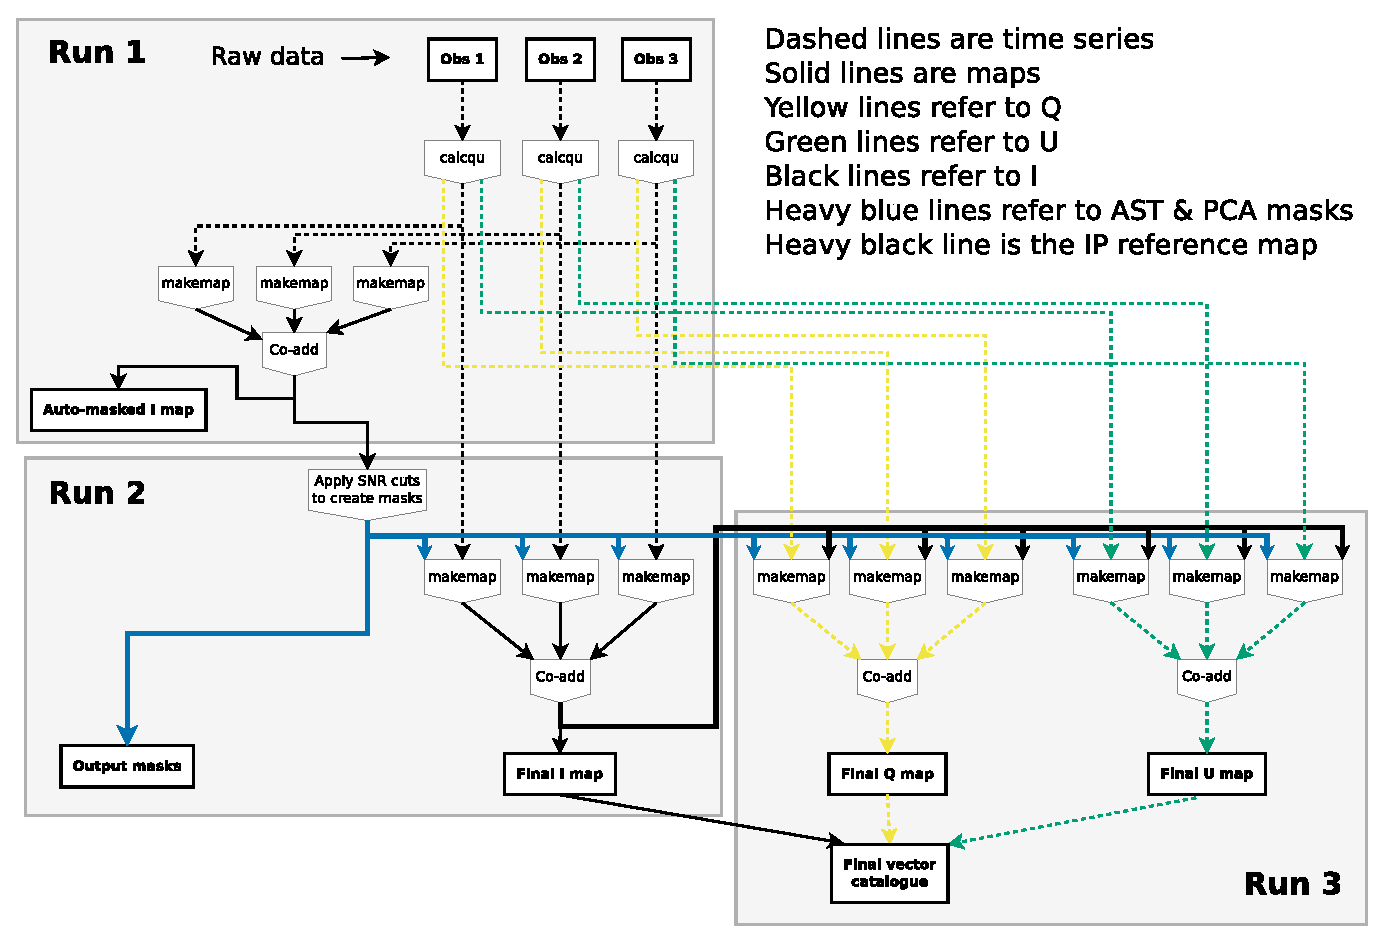
\includegraphics[width=.99\linewidth]{figs/pol2map_flow.eps}
\caption{The \texttt{pol2map} data flow for the case of three
observations being processed. Each grey box refers to a single invocation
of \texttt{pol2map}.}
\label{fig:flow}
\end{figure}

The main themes of the processing are:

\begin{itemize}
\item The \texttt{makemap} configuration has been tailored to ensure that
usable maps are created from the I time-streams created by \texttt{calcqu}.
\item The same configuration is also used to create maps from the Q and U
time-streams. This is to ensure consistency between the I, Q and U maps.
\item The IP corrections applied to the Q and U data are based on the I
map made from the same POL2 data, and in the same way, as the Q and U maps.
\item The same masks used to create the I maps are also used to create
the Q and U maps.
\item The calculation of fractional polarisation values are based on I, Q
and U maps made from the same data and made in the same way.
\end{itemize}

As with the older \texttt{pol2scan} script, the processing performed by
\texttt{pol2map} can be divided into two section:

\begin{itemize}
\item The creation of time-stream files holding Q, U and I values from
the raw data holding analysed intensity time-streams for each bolometer.
This stage is performed by the \texttt{smurf:calcqu} command. The
resulting Q, U and I time-streams are sampled at 2 Hz.
\item The creation of two-dimensional maps from these Q, U and I
time-streams. This stage is performed by the \texttt{smurf:makemap} command.
Note, unlike \texttt{pol2scan}, \texttt{pol2map} creates maps from the I
time-streams as well as the Q and U time-streams.
\end{itemize}

Most of the differences between \texttt{pol2scan} and \texttt{pol2map}
relate to the second section, specifically the configuration parameters
and masking options that are used when running \texttt{makemap}. The most
significant difference from the point of view of using the script is the manner
in which masks are defined and used.

\subsection{Masking}
A mask is a two-dimensional array which has the same shape and size as
the final map, and which is used to indicate where the source is expected
to fall within the map. Bad pixel values within a mask indicate
background pixels, and good pixels values indicate source pixels. Masks
are used for two main purposes:

\begin{enumerate}
\item To prevent the growth of gradients and other artificial large scale
structures within the map. For this purpose, the astronomical signal at
all background pixels defined by the mask is forced to zero at
the end of each iteration within \texttt{makemap} (except for the final
iteration).
\item To prevent bright sources polluting the evaluation of the various
noise models (PCA, COM, FLT) used within \texttt{makemap}. Source pixels
are excluded from the calculation of these models.
\end{enumerate}

The \texttt{pol2map} script uses different masks for these two purposes -
the ``AST'' mask and the ``PCA'' mask\footnote{The PCA mask is also used
to mask the COM and FLT models.}. The PCA mask is in general less
extensive than the AST mask, with the source areas being restricted to
the brighter inner regions.

Each of these two masks can either be generated automatically within
\texttt{makemap}, or be specified by a fixed external NDF. In addition,
the masks can be defined as a circle of known radius centred on the
expected source position. If the mask is generated automatically within
\texttt{makemap}, it is created by applying a cut to the signal-to-noise map
at the end of each iteration. The ``auto-mask'' cut levels used by
\texttt{pol2map} are:

\begin{description}
\item[AST]: An initial cut is made at an SNR of 3.0 but each resulting
contiguous source region is then extended down to an SNR of 2.0.
\item[PCA]: An initial cut is made at an SNR of 5.0 but each resulting
contiguous source region is then extended down to an SNR of 3.0.
\end{description}

A new mask is created at the end of each iteration, and so the mask can
change from iteration to iteration. The benefit of using auto-masking is
that no previous map of the sky is required. The disadvantage is that
different maps of the same region can be processed with different masks.
This is significant as the AST mask defines the region in which
significant emission is allowed to grow, and so using different masks can
result in non-uniform processing of multiple observations of the same
region. It is thus beneficial to process all observations of a single
object using the same mask. This suggests a two stage process in which
the I time-streams for all available observations are processed initially
using the auto-masking method. These initial ``auto-masked'' maps are
then co-added to produce an I map with higher signal-to-noise. A new mask
is then defined by applying an SNR cut to this I co-add. All I
time-streams are then re-processed by \texttt{makemap} a second time
using this static mask to define the source regions for all observations.
The resulting ``externally-masked'' I maps are then co-added to produce
the final I co-add.

The Q time-streams are then processed by \texttt{makemap}, using the same
external static mask that was used to produce the final I maps. In
addition, the final co-added I map is used to define the expected levels
of Instrumental Polarisation when doing IP correction. The Q maps for
individual observations are co-added to form the final Q map. The U
time-streams are then processed in exactly the same way to produce the
final U map. The final I, Q and U maps are then combined to form the
vector catalogue. This entire process is illustrated in
Fig.\ref{fig:flow}.

\subsubsection{Mask creation}
The AST and PCA masks are derived from the signal-to-noise map
($Data/\sqrt(Variance)$) created from the co-add of the auto-masked I
maps from all observations.  The \emph{FellWalker} algorithm provided by the
\texttt{cupid:findclumps} program is used to define the source regions within
the SNR map. Each source region within the AST mask consists of a contiguous
group of pixels above an SNR of 2.0, with at least one pixel having an SNR
above an SNR of 3.0. The following configuration is used with
\texttt{findclumps}:

\begin{quote}
\begin{verbatim}
FellWalker.FlatSlope=0
FellWalker.MinDip=1.0E30
FellWalker.Noise=2.0
FellWalker.MinHeight=3.0
\end{verbatim}
\end{quote}

The PCA mask is formed in the same way but the SNR limits are changed so
that each source region consists of a contiguous group of pixels above an
SNR of 3.0, with at least one pixel having an SNR above an SNR of 5.0.

For some very bright astronomical sources such as Orion A, the resulting
source areas can occupy the majority of the map. This causes problems
within \texttt{makemap}, because such large source regions applies little
constraint on the development of gradients and other large scale
structures. In addition, blanking out such large areas of sky when
forming the noise models can result in the noise models being poorly
defined.

To avoid these problems, a check is made on the AST mask to ensure it is
not too large. If the source regions in the AST mask occupy more than
20\% of the map, then a new mask is formed using slightly higher SNR
limits. This process repeats until an SNR limits are found which result
in no more than 20\% of the map pixels being designated as source pixels.

A similar process is applied to the PCA mask, but here the restriction is
that the source regions occupy no more than 10\% of the map.

The masks actually used can be saved to disk by assigning values to the
MASKOUT1 and MASKOUT2 parameters when running \texttt{pol2map}.

\subsubsection{Mask usage}

When \texttt{pol2map} is run with parameter MASK set to ``AUTO'', new
AST and PCA masks are created automatically at the end of each iteration.
Under certain circumstances this can prevent convergence of the
\texttt{makemap} iterative process, due to marginal pixels at the edge of
a source repeatedly entering then leaving the mask. To avoid this, the AST
mask is frozen when the normalised change in the map between iterations
falls below 0.2 (\texttt{ast.zero\_freeze = 0.2}).

In addition, when using auto-masking, an initial set of ten iterations
are performed in which the astronomical signal is \emph{not} removed at
the end of the iteration (\texttt{ast.skip = 10}). This allows initial PCA
and AST masks to be created before the genuine iterative process begins,
which speeds up convergence significantly.

When using either auto-masking or external-masking, the masking of noise
models using the PCA mask is only performed up to the point where the
normalised map change between iterations falls below 0.5
(\texttt{pca.zero\_niter = 0.5}, \texttt{com.zero\_niter = 0.5},
\texttt{flt.zero\_niter = 0.5}). By this point, most of the astronomical
signal should have been moved out of the time-streams and into the map,
resulting in there being little point in masking the time-streams.

\subsection{Convergence testing}

Each invocation of \texttt{makemap} continues to converge until the
maximum normalised change between iterations in any map pixel is less
than 0.05 (\texttt{maptol = 0.05},\texttt{maptol\_mean = 0}). The map
change is first smoothed using a  box filter of size 60 arc-seconds before
finding the maximum map change value (\texttt{maptol\_box = 60}). Edge pixels
(\emph{i.e.} pixels that contain fewer than the mean number of bolometer
samples) are not included in the check - \texttt{maptol\_hits = 1.0}.

This scheme ensures that convergence is not affected by the size of the
source regions. For instance, using the usual scheme based on the mean
map change within the source region (\texttt{maptol\_mean = 1}), no further
iterations are performed if no pixels reach the SNR limit for the AST mask
(\texttt{ast.zero\_snr}) at the end of the first iteration. This
is inappropriate given the use of the PCA model within \texttt{pol2map},
since (unlike other models such as COM or FLT) the PCA model only passes
through a fraction of the astronomical signal on each iteration. Thus,
curtailing the iterative process after only one iteration would mean loosing
astronomical flux that might make it through into the map if further
iterations were performed.

\subsection{Iterative models}

The old \texttt{pol2scan} script used just the PCA (Principal Component
Analysis) model to identify and remove sky and electronic background
signals from the I, Q and U time-stream values when running
\texttt{makemap}. Improved results seem possible --- particularly when
processing I time-streams, which usually have much stronger signals than the
Q or U time-streams --- if the PCA model is preceded by a COM
(common-mode) model, and followed by a FLT (high-pass filter) model. This
the model order used is \texttt{modelorder=(com,gai,pca,ext,flt,ast,noi)}

The PCA model identifies and removes a specified number of template
time-stream backgrounds from the data, where the strength of the template
can change from bolometer to bolometer. It choose the templates to be the
time-streams that are most correlated with the existing bolometer data.
The more components (i.e. background time-streams) that are removed, the
less background noise there is in the final map, but the longer the map
takes to produce. This is because removing many components usually
results in some of the astronomical signal being removed from the data, in
addition to the correlated background noise. This in turn means that more
iterations are required to recover the full astronomical signal. This is
different to the COM or FLT components, which pass the full astronomical
signal on each iteration.

By default, if auto-masking is used, the strongest 50 PCA components are
removed on each iteration. If external-masking is used, the strongest 150
PCA components are removed by default on each iteration. The reasoning
for this difference is that speed is more important than accuracy when
forming the initial auto-masked map, since the auto-masked map is only
used to create the masks used to create subsequent external-masked maps.
These defaults may be lowered if the high initial values prevent maps
from converging - see the next section.

\subsection{Convergence}
An upper limit of 200 is placed on the number of iterations to be
performed. If a map has not converged to the required MAPTOL (0.05 by
default) within this number of iterations, the resulting map may not
accurately represent the bright emission in the field. The level of
inaccuracy is very hard to quantify but will depend on how far from
convergence the map was when the limit of 200 iterations was reached. It
is therefore a good idea to check that maps did in fact converge. This
can be done by searching the \texttt{pol2map} log file for the string
``\texttt{Solution did NOT converge}''. If this string is found within
the log file, the level of convergence achieved before \texttt{makemap}
exited can be found by searching backwards through the log file for the
previous occurrence of the string ``\texttt{NORMALIZED MAP CHANGE:}''. For
instance:

\begin{quote}
\begin{verbatim}
smf_iteratemap: *** NORMALIZED MAP CHANGE: 0.0501144 (mean) 0.3485134 (max)
\end{verbatim}
\end{quote}

The second value (0.3485134 in the above example) shows the level of
convergence that was achieved. This number should be compared to the
MAPTOL value (0.05 by default) to determine how far the solution is from
convergence.

Achieving convergence takes longer for bright sources than for faint
sources. This is mainly because of the PCA model that is used within
\texttt{pol2map}. The number of iterations required for convergence goes
up as the number of PCA components removed on each iteration goes up. For
very bright sources, the default values of PCA.PCATHRESH may be too high
too allow convergence to be reached within 200 iterations\footnote{This
is only usually a problem for I maps, since the source is much fainter in
Q and U maps.}. Increasing the maximum number of iterations is possibly
one way to correct this. However, in some cases it may be necessary to
perform many hundreds or even thousands of iterations to achieve
convergence, which could take days or weeks to run on a typical SCUBA-2
PC. This is usually impractical and so the alternative solution of
reducing the number of removed PCA components when creating new maps is
implemented within \texttt{pol2map} using the following scheme:

\begin{enumerate}
\item If the user specifies a value for PCA.PCATHRESH using the CONFIG
parameter, that value is always used. Note, the number of iterations to
remove must be given as a negative value. Thus a value of -150 means
``remove 150 PCA components''.
\item Otherwise, if any previously created maps of the same kind (\emph{i.e.}
auto-masked or externally-masked) already exist in the output maps directory,
then the PCA.PCATHRESH value used to create the most recent of those maps is
re-used to create the new maps.
\item Otherwise, if we are creating new externally-masked maps, and the
output maps directory contain some previously created auto-masked maps,
then the PCA.PCATHRESH value used to create the most recent of those
auto-masked maps is re-used to create the new externally-masked maps,
\emph{but only if that value is less than the default auto-mask value of
50}. The rationale for this is that if it was found necessary to reduce
the number of removed PCA components when creating the auto-masked maps,
then it will also be necessary to do the same with the externally-masked
maps. But on the other hand, if the auto-masked maps were created successfully with the default
value of PCA.PCATHRESH, then it may be possible to increase the number of
removed PCA components and still achieve convergence. This is one of the
goals when using external-masking, in order to achieve lower noise maps.
\item Otherwise (\emph{i.e.} if we cannot determine a PCA.PCATHRESH value
from any previously created maps), we initially use the default value for
PCA.PCATHRESH (-50 for auto-masking and -150 for external-masking) but
include a check on convergence when \texttt{makemap} is run to create a
map from the first supplied observation. If \texttt{makemap} fails to
converge within 200 iterations using the default PCA.PCATHRESH value, the
value is reduced by $25\%$ and \texttt{makemap} is re-run. The same check
is performed again and \texttt{makemap} re-run with a reduced
PCA.PCATHRESH if convergence has still not been achieved. This process
continues until convergence is achieved, or a lower limit (-5) is reached
for PCA.PCATHRESH. Messages displayed on standard output indicate the
success or failure of each used PCA.PCATHRESH value. Having determined a
value for PCA.PCATHRESH that allows convergence to be reached for the
first supplied observation, the same value is used for all subsequent
observations. This process is speeded up by allowing \texttt{makemap} to
abort early (\emph{i.e.} before 200 iterations have been completed) as
soon as it becomes likely that convergence will not be reached within 200
iterations. This decision is taken on the basis of the fall in the
normalised map change seen over the initial iterations. This fall is
assumed to be exponential in form, allowing the curve of ``map change''
versus ``iteration number'' to be modelled and extrapolated. This allows
\texttt{makemap} to form an estimate of the iteration number at which the
required MAPTOL value will be reached.
\end{enumerate}

The disadvantage of achieving convergence by reducing the PCA.PCATHRESH
value is that the resulting maps will have a noisier background with more
bowling around bright sources.

\section{IP correction}
The existing IP correction (referred to as ``PL2'') is based on the mean I, Q
and U values of Uranus observed over a range of elevations. The Q and U
values were created from POL2 observations using a method similar to
\texttt{pol2scan}. The I values were created from non-POL2 observations
using \texttt{makemap} directly. The PL2 IP model does not take the POL2
degradation factor into account - this is so that it can be applied
directly to the IP reference map supplied to pol2scan, which until now
has always been a non-POL2 map. A change has been made to
\texttt{makemap} so that when using the PL2 model, it now detects whether
the IP reference map was created from POL2 data, and if so, multiplies it
by the canonical POL2 degradation factor at 850 $\mu m$ (1.35).

In addition, an entirely new IP model called ``PL3'' has been created
from the same set of Uranus observations. The Q, U and I maps were all
made from POL2 data using a circular mask of 30 arc-seconds radius and a
\texttt{makemap} configuration similar to that used by \texttt{pol2map}
in ``external mask'' mode. It was necessary to remove the COM model, as
including the COM model made the scatter of Q and U values about the fit
much larger.

The plots in this section compares the measured and fitted values for the
basic parameters of PL2 and PL3. Figures~\ref{fig:ip1} and~\ref{fig:ip2}
show that the overall level of instrumental polarisation is higher in PL3
than in PL2. This is because PL3 takes account of the POL2 degradation
when forming the fractional polarisation (by virtue of the fact that the
I values are derived from POL2 data), whereas PL2 does not. By default,
\texttt{makemap} now uses the PL3 model if the IP reference map was
created from POL2 data, and the PL2 model otherwise.

It is disappointing that the scatter of the measured values around the
fit are if anything worse in PL3 than in PL2, given the significant
reduction in the noise visible in the maps created using \texttt{pol2map}
and presented in section~\ref{sec:results}.

\begin{figure}
\centering
\begin{minipage}{.45\textwidth}
  \centering
  \includegraphics[width=.95\linewidth]{ip/fig1}
  \captionof{figure}{The measured mean Q values in PL2 (red) and PL3 (blue)}
\end{minipage}
~~
\begin{minipage}{.45\textwidth}
  \centering
  \includegraphics[width=.95\linewidth]{ip/fig2}
  \captionof{figure}{The measured mean U values in PL2 (red) and PL3 (blue)}
\end{minipage}
\end{figure}


\begin{figure}
\centering
\begin{minipage}{.45\textwidth}
  \centering
  \includegraphics[width=.95\linewidth]{ip/fig3}
  \captionof{figure}{The measured fractional polarisation values in PL2 (red) and PL3 (blue)}
  \label{fig:ip1}
\end{minipage}
~~
\begin{minipage}{.45\textwidth}
  \centering
  \includegraphics[width=.95\linewidth]{ip/fig4}
  \captionof{figure}{The fitted  fractional polarisation values in PL2 (red) and PL3 (blue)}
  \label{fig:ip2}
\end{minipage}
\end{figure}


\begin{figure}
\centering
\begin{minipage}{.45\textwidth}
  \centering
  \includegraphics[width=.95\linewidth]{ip/fig5}
  \captionof{figure}{The measured polarisation angles in PL2 (red) and
                     PL3 (blue), with respect to the focal plane Y axis.}
\end{minipage}
~~
\begin{minipage}{.45\textwidth}
~~
  \centering
\end{minipage}
\end{figure}


\section{Example results from \texttt{pol2map} compared to \texttt{pol2scan}\label{sec:results}}
This section presents some very preliminary results produced by
\texttt{pol2map} for a range of different extended astronomical objects,
and compares these with equivalent results produced using the old
\texttt{pol2scan} script.

Note, these results have not been verified completely - there may be
serious issues present that need addressing within the software. These
reductions should be repeated by other people, and some independent
verification and analysis performed.

The same automatically generated plots are shown for each object:
\begin{enumerate}
\item Q and U maps: \texttt{pol2scan} maps followed by \texttt{pol2map}
maps with and without IP correction.
\item Q and U Signal-to-Noise maps: \texttt{pol2scan} maps followed by
\texttt{pol2map} maps with and without IP correction.
\item Q/U pixel errors (central region only): scatter plots compare
\texttt{pol2scan} error values compared to \texttt{pol2map}.
\item I map errors compared to Q/U map errors: all from \texttt{pol2map}
\item pol2map I map compared to non-POL2 SCUBA-2 map: two display scales
are used to highlight the bright regions and the faint regions for
comparison. The non-POL2 maps are corrected using the canonical
degradation factor (1.35 at 850 $\mu m$) before being displayed. A
difference map is included - ideally this would be a smooth map
containing just the extra extended structure present in the non-POL2 maps
but not present in the POL2 maps. In fact the presence of small scale
structures suggest he degradation factor of 1.35 may not always be
appropriate.
\item Polarised intensity maps: these are binned 3x3 to produce 12
arc-second pixels. The de-biased maps contain many bad pixels (shown in
grey) where the polarised intensity is less than the noise.
\item Polarised intensity Signal-to-Noise maps: also binned to create 12
arc-second pixels.
\item De-biased vector maps - binned 5x5 and cut at $(dp<3)\&\&(dang<10)$
\end{enumerate}

The red contours shown in some images indicate the areas that were used
to create the associated statistics or plots shown on the same page. All
maps shown on a single page share the same display scale, unless
otherwise noted.

Points to note:
\begin{enumerate}
\item The time taken to process a set of observations using
\texttt{pol2map} can be five times more than using \texttt{pol2scan}.
\item The backgrounds in the Q and U produced by \texttt{pol2map} are much
flatter and have around $30\%$ less noise than the equivalent maps
produced by \texttt{pol2scan}.
\item The on-source SNR values are higher for \texttt{pol2map} than for
\texttt{pol2scan}.
\item The errors in the I pixel values created from POL2 data are similar
in magnitude to the Q and U errors created from the same data. This means
that performing IP correction with these I maps will not add
significantly  to the noise in the final maps.
\item The I maps created from POL2 data have flatter backgrounds than
those created from non-POL2 data.
\item The I maps created from POL2 data have a higher NEFD than those
created from non-POL2 data.
\end{enumerate}



\subsection{Serpens - field 1}
These maps are made from 21 observations of Serpens field 1 taken
between 20160420 and 20160522.

\includepdf[pages={-}]{figs/fig2.pdf}
\includepdf[pages={-}]{figs/fig3.pdf}
\includepdf[pages={-}]{figs/fig4.pdf}
\includepdf[pages={-}]{figs/fig5.pdf}
\includepdf[pages={-}]{figs/fig6.pdf}
\includepdf[pages={-}]{figs/fig7.pdf}
\includepdf[pages={-}]{figs/fig8.pdf}
\includepdf[pages={-}]{figs/fig9.pdf}

\subsection{G34}
These maps are made from 4 observations of G34 taken on 20160729.

\includepdf[pages={-}]{figs/fig11.pdf}
\includepdf[pages={-}]{figs/fig12.pdf}
\includepdf[pages={-}]{figs/fig13.pdf}
\includepdf[pages={-}]{figs/fig14.pdf}
\includepdf[pages={-}]{figs/fig15.pdf}
\includepdf[pages={-}]{figs/fig16.pdf}
\includepdf[pages={-}]{figs/fig17.pdf}
\includepdf[pages={-}]{figs/fig18.pdf}

\subsection{IC 5146}
These maps are made from 19 observations of IC 5146 taken between
20160523 and 20160910.

\includepdf[pages={-}]{figs/fig20.pdf}
\includepdf[pages={-}]{figs/fig21.pdf}
\includepdf[pages={-}]{figs/fig22.pdf}
\includepdf[pages={-}]{figs/fig23.pdf}
\includepdf[pages={-}]{figs/fig24.pdf}
\includepdf[pages={-}]{figs/fig25.pdf}
\includepdf[pages={-}]{figs/fig26.pdf}
\includepdf[pages={-}]{figs/fig27.pdf}


\subsection{DR 21}
These maps are made from 13 observations of DR 21 taken between 20150716 and
20150918.

\includepdf[pages={-}]{figs/fig29.pdf}
\includepdf[pages={-}]{figs/fig30.pdf}
\includepdf[pages={-}]{figs/fig31.pdf}
\includepdf[pages={-}]{figs/fig32.pdf}
\includepdf[pages={-}]{figs/fig33.pdf}
\includepdf[pages={-}]{figs/fig34.pdf}
\includepdf[pages={-}]{figs/fig35.pdf}
\includepdf[pages={-}]{figs/fig36.pdf}


\subsection{Perseus b1}
These maps are made from 8 observations of Perseus b1 taken between
20160908 and 20160911.

\includepdf[pages={-}]{figs/fig38.pdf}
\includepdf[pages={-}]{figs/fig39.pdf}
\includepdf[pages={-}]{figs/fig40.pdf}
\includepdf[pages={-}]{figs/fig41.pdf}
\includepdf[pages={-}]{figs/fig42.pdf}
\includepdf[pages={-}]{figs/fig43.pdf}
\includepdf[pages={-}]{figs/fig44.pdf}
\includepdf[pages={-}]{figs/fig45.pdf}

\subsection{Ophiuchus - field 3}
These maps are made from 18 observations of Ophiuchus field 3 taken between
20160522 and 20160910.

\includepdf[pages={-}]{figs/fig47.pdf}
\includepdf[pages={-}]{figs/fig48.pdf}
\includepdf[pages={-}]{figs/fig49.pdf}
\includepdf[pages={-}]{figs/fig50.pdf}
\includepdf[pages={-}]{figs/fig51.pdf}
\includepdf[pages={-}]{figs/fig52.pdf}
\includepdf[pages={-}]{figs/fig53.pdf}
\includepdf[pages={-}]{figs/fig54.pdf}

\subsection{Orion A}
These maps are made from 20 observations of Orion A taken between 20160111
and 20160125.

\includepdf[pages={-}]{figs/fig56.pdf}
\includepdf[pages={-}]{figs/fig57.pdf}
\includepdf[pages={-}]{figs/fig58.pdf}
\includepdf[pages={-}]{figs/fig59.pdf}
\includepdf[pages={-}]{figs/fig60.pdf}
\includepdf[pages={-}]{figs/fig61.pdf}
\includepdf[pages={-}]{figs/fig62.pdf}
\includepdf[pages={-}]{figs/fig63.pdf}

\section{Future work}

\begin{itemize}
\item Further verification of the results presented in section~/ref{sec:results}.
\item As yet no attempt has been made to determine whether these results are
consistent with the canonical value of 1.35 for the POL2 degradation factor at 850
$\mu m$. This could be done by comparing I maps of points sources
created from POL2 observations using \texttt{pol2map}, with maps made
from non-POL2 data using \texttt{makemap} directly. Point sources need to
be used rather than extended sources to avoid complexities caused by the
different spatial frequencies present in POL2 and non-POL2 observations.
\item A more extensive investigation of the NEFD present within POL2 I
maps needs to be performed.
\end{itemize}

\appendix
\section{Using \texttt{pol2map} on simulated POL2 data}

This section compares maps made by \texttt{pol2map} from simulated POL2
data, with the known astronomical I, Q and U maps from which the
simulated data were generated. The main purpose is to investigate the
following questions:

\begin{itemize}
\item Are the FCFs for the reconstructed I maps the same as those for the
reconstructed Q and U maps? If so, the FCF will cancel out when forming
fractional polarisations and angles, and so becomes unnecessary for most
purposes\footnote{The exception is if the polarised intensity, in Jy, is
the quantity of scientific interest.}.
\item Do the reconstructed I, Q and U maps contain the same spatial
frequencies? This is desirable if the I maps are used to perform IP
correction on the Q and U maps.
\item How does the noise, FCF and spatial frequency response change as you
change the PCA.PCATHRESH value?
\end{itemize}

The final conclusions section in this appendix contains a summary of the
answers to these questions.

\subsection{The simulated data}
The known I map from which the simulated POL-2 values are generated contains
a single Gaussian blob of emission. Many separate simulations were
performed in which the size and brightness of the blob were varied. The
known Q and U maps were generated from the known I map assuming a
constant polarisation of 5\% parallel to the reference
direction\footnote{Thus the known U value is always zero.}.

The simulated data is created using a real POL2 observation as a template
to define the half-wave plate position and sky position associated with
each bolometer sample. The observation used was observation 50 from
20160508 - a POL2 observation of CB 68. This is not quite  a blank field,
but the levels of astronomical Q and U seen in this observation are
barely significant. However, care is taken to exclude the real astronomical
signal present in the template observation when comparing the
reconstructed I, Q and U maps with the known I , Q and U maps described
above.

Multiple simulations were performed in which the size and strength of the
Gaussian blob were varied\footnote{The noise is constant across all
simulations since it is defined by the template observation.}. In addition,
for each size and strength
combination, \texttt{pol2map} was run five times using different values
for the PCA.PCATHRESH parameter\footnote{A notional value of zero for PCA.PCATHRESH
is used to indicate that no PCA model was used.}. The following values were used:

\begin{description}
\item[Source FWHM (arc-seconds):] 16, 32, 48, 64, 80, 96, 112, 128
\item[Source strength (SNR):] 10, 30, 100, 300, 1000, 3000, 10000
\item[PCA.PCATHRESH:] 0, 10, 50, 100, 150
\end{description}

Note, the source strengths above were converted from SNR to pW assuming a
noise value of 2E-5 pW - the noise measured in maps made from the
template observation alone. A pixel size of 4 arc-sec was used for all
maps. A simulation was performed for each combination of the above values,
resulting in a total of $8\times7\times5 = 280$ simulations.

For each simulation, the following procedure was followed:

\begin{enumerate}
\item Select the combination of source size, source strength and
PCA.PCATHRESH values to use in the simulation.
\item Use \texttt{pol2map} twice to create maps of the real I, Q and U present
in the template observation alone. These maps are created using a 2-step
process: firstly, an auto-masked I map is created using the default value
for PCA.PCATHRESH provided by \texttt{pol2map} (-50), secondly,
externally-masked I, Q and U maps are created using the auto-masked I map
to define the AST mask used by all three maps. The Q and U maps have IP
correction based on the externally-masked I map. These externally masked
maps are created using the PCA.PCATHRESH value associated with the
current simulation. No extinction
correction is used. This is so that the resulting maps can be compared
directly with the maps generated later from the simulated data, which do
not include extinction correction.
\item Generate an artificial I map holding a noise free Gaussian blob with
the current value for source size (FWHM) and source strength. This blob
is centred at the expected  position of CB 68 in the I map created in the
previous step.
\item Generate maps of artificial Q and U from the above artificial I map,
assuming a polarisation of 5\% parallel to the reference direction (the pixel
Y axis).
\item For each bolometer sample in the template observation, get
the I, Q and U values from the corresponding pixel in the above
artificial maps using \texttt{sincsinc} interpolation \footnote{Random
pointing errors of 1.0 arc-second are introduced here.}. Combine these
three values into an analysed intensity value using the half-wave
plate position associated with the bolometer sample. A perfect polarimeter
is assumed:

\[ I_{rec} = \frac{1}{2}( I + Q.\cos 2\phi + U.\sin 2\phi ) \]

where $I_{rec}$ is the recorded analysed intensity and $\phi$ is the
angle between the rotated plane of polarisation and the HWP fast axis
(i.e. $\phi = 2.WPLATE$). Instrumental
Polarisation is added based on the ``PL3'' IP model and the I values. Add
this artificial analysed intensity value onto the existing real bolometer
value in the template observation. Note, the artificial data value is
\emph{not} modified to take account of atmospheric extinction.

\item Use the \texttt{pol2map} command twice to generate I, Q and U
maps from the analysed intensity time-streams generated in the previous
step (\emph{i.e.} these maps include both the real CB 68 signal, plus the
signal from the artificial source). The same two-step map-making process is
used as described for the real data in step 2.

\item The real I map generated at step 2 from the template data alone is
subtracted from the I map created in the previous step. This leaves the I
map holding data purely from the artificial Gaussian blob alone (see
Fig.~\ref{fig:icor}). Likewise the real Q and U data are removed from the
Q and U maps.

\begin{figure}
\includegraphics[width=0.9\columnwidth]{figs/icor}
\caption{Total intensity maps from the simulation for FWHM=16 SNR=30
PCATHRESH=150. Bottom left map is the template observation alone. Bottom
right map is the original simulated source. Top left is the reconstructed
map made from the template observation and the simulated data. Top right
is the residual map left after the bottom left map is subtracted from the
top left map (\emph{i.e.} the reconstructed simulated source). }
\label{fig:icor}
\end{figure}

\item The total source signal in the reconstructed I, Q and U maps generated by the
previous step are found by summing the pW pixel values within a circle of
diameter twice the source FWHM, centred on the expected source centre.
Likewise, the  total source signal in the artificial  I, Q and U maps are
found using the same aperture. These value allow the I, Q and U gains to
be found. For instance, the I gain is the total value within the aperture
in the reconstructed I map divided by the  total value within the same aperture
in the artificial I map.

\item The pol2map log files are parsed to discover the number of
iterations that were performed when creating the reconstructed I map,
and the normalized map change on the penultimate iteration.

\end{enumerate}

The end result is a table in which the columns are:

\begin{itemize}
\item Original source size (FWHM in pixels)
\item Original source strength (SNR)
\item PCA.PCATHRESH used to create the externally-masked reconstructed maps
\item I gain (total source I in reconstructed map divided by total source I in artificial map)
\item Q gain (total source Q in reconstructed map divided by total source Q in artificial map)
\item Number of iterations
\item Final normalized map change
\end{itemize}

No U gain column is created because the U values in the artificial maps
are always zero, due to the choice of polarisation angle in the artificial
data. The table contains one row for each combination of original source size,
strength and PCATHRESH value - a total of 280 rows. This table may be
downloaded from
\htmladdnormallink{http://www.eao.hawaii.edu/~dberry/pol2sim.asc}
{http://www.eao.hawaii.edu/~dberry/pol2sim.asc}, and explored using:

\begin{verbatim}
% topcat -f ascii pol2sim.asc
\end{verbatim}

\subsection{Results and Analysis}

The first step in the analysis is to identify and remove the simulations
in which the reconstructed I map did not reach convergence within 200 iterations (there
were 54 such simulations - see Fig.~\ref{fig:converged}. The un-converged
simulations are predominantly at the bright end of the source strength
axis, with larger sources taking longer to converge than smaller sources.
Also, higher values of PCA.PCATHRESH take longer to converge.

\begin{figure}
\includegraphics[width=0.9\columnwidth]{figs/converged}
\caption{Simulations that failed to converge in 200 iterations (red dots
are converged, blue dots are un-converged). The left-right axis is source
strength (logarithmic), the up-down axis is PCA.PCATHRESH and the in-out axis is source
size.}
\label{fig:converged}
\end{figure}

One of the assumptions behind \texttt{pol2map} is that the FCF in the I,
Q and U maps are all the same and so can be discounted when calculating
the fractional polarisation. To test this assumption.
Fig.~\ref{fig:iqgain} shows a scatter plot of the Q gain against the I
gain in the table described above. It can be seen that the I and Q gains
are approximately equal, except for noise, with a strong tendency
to cluster around unity. However, the scatter in this plot is surprisingly
high. The cause of this scatter is currently unknown.

Figures~\ref{fig:iqgain-snr}, \ref{fig:iqgain-ssize} and
\ref{fig:iqgain-pt} show the same data, but use colour to indicate the
source SNR, source size and PCA threshold used. They show that large,
faint sources have a low gain. This is confirmed in figures~\ref{fig:igain}
and \ref{fig:qgain}. Fig.~\ref{fig:iqgain-pt} may suggest that the Q gain
tends to be lower than the I gain for low PCA thresholds - particularly
if no PCA model is used at all (i.e. zero threshold).

So the answer to the first question posed as the start of this appendix -
``are the FCFs for the reconstructed I maps the same as those for the
reconstructed Q and U maps?'' - is yes, to within a certain degree.
Fig.~\ref{fig:ratio} quantifies this by showing a histogram of the ratio
of the Q gain to the I gain. After removal of out-liers, this
distribution has a mean of 1.05 and a standard deviation of 0.13.
Fig.~\ref{fig:ratio-pt} plots the mean ratio (averaged over all source
sizes and strengths) at each PCA threshold, together with one sigma error
bars. This plot suggests that the ratio deviates from unity significantly
at higher PCA thresholds, and also that the ratio has greater noise at
higher PCA thresholds. This result may suggest that a PCA threshold of 50
would produce more consistent and accurate results than the current
default value of 150\footnote{However, making this change would increase
the background noise level.}. For PCA threshold of 50, the mean ratio
(after removal of out-liers) is 1.03 and the standard deviation is 0.09.

Since the map-making process within pol2map produces seemingly random
changes in FCF for simulated data, it is likely that it will also produce
similar changes for real data, which will lead to errors in the
fractional polarisation created by pol2map. If

\[ r = \frac{Gain_{Q}}{Gain_{I}} \]

then

\[ P_{measured} = P_{actual} . r \]

So the variance on the measure polarisation is increased by the variance
in $r$:

\[ \sigma^2_{Pm} = \sigma^2_{Pa}.r^2 + \sigma^2_r.P^2_{actual} \]

Approximating the mean ratio by 1.0, and noting that $\sigma_r$ is 0.13,
this means that the error in the fractional polarisation should be
increased from $dP$ to $dp'$, where:

\[ dP'  = \sqrt{ dP^2 + 0.017.P^2 } \]

For instance, a 5\% vector that has an original error of 1\% should have
its error increased to 1.2\%. If we swapped to using a PCA
threshold of 50, for which $\sigma_r$ is 0.09, the above equation becomes:

\[ dP'  = \sqrt{ dP^2 + 0.008.P^2 } \]

and the increased error for the 5\% example vector would become  1.1\%.

However, this increase in the error should only be done within
pol2map if the MAPVAR parameter is set False (\emph{i.e.} output
variances are derived by propagating the variances calculated by
\texttt{makemap}). If MAPVAR is True, then the output variances are derived from
the spread of values from all observations at each point on the sky, and
thus the random fluctuations in FCF described above will already be taken
into account.




\begin{figure}
\includegraphics[width=0.9\columnwidth]{figs/iqgain}
\caption{The gain seen in the reconstructed I and Q source strengths. A
value of 1.0 means that the source has the same strength in the
reconstructed map as in the original artificial source map. The
reconstructions that failed to converge are omitted from this plot. The
line of grey dots indicate the desired one-to-one line}
\label{fig:iqgain}
\end{figure}


\begin{figure}
\includegraphics[width=0.9\columnwidth]{figs/iqgain-snr}
\caption{The gain seen in the reconstructed I and Q source strengths,
coloured by source strength.}
\label{fig:iqgain-snr}
\end{figure}


\begin{figure}
\includegraphics[width=0.9\columnwidth]{figs/iqgain-ssize}
\caption{The gain seen in the reconstructed I and Q source strengths,
coloured by source size.}
\label{fig:iqgain-ssize}
\end{figure}

\begin{figure}
\includegraphics[width=0.9\columnwidth]{figs/iqgain-pt}
\caption{The gain seen in the reconstructed I and Q source strengths,
coloured by PCA threshold.}
\label{fig:iqgain-pt}
\end{figure}

\begin{figure}
\includegraphics[width=0.9\columnwidth]{figs/ratio}
\caption{A histogram of the ratio of Q gain to I gain.}
\label{fig:ratio}
\end{figure}

\begin{figure}
\includegraphics[width=0.9\columnwidth]{figs/ratio-pt}
\caption{The mean ratio of Q gain to I gain, at different PCA thresholds,
with a-sigma error bars.}
\label{fig:ratio-pt}
\end{figure}



Fig.~\ref{fig:igain} shows the I gain (shown by colour) as a function of source strength,
source size and PCA.PCATHRESH value. It can be seen that:

\begin{itemize}
\item the I gain becomes smaller at larger source sizes and smaller
source strengths.
\item there is no clear dependence on PCA.PCATHRESH.
\end{itemize}

\begin{figure}
\includegraphics[width=0.9\columnwidth]{figs/igain}
\caption{The I gain (shown by colour) as a function of source strength, size and
PCA.PCATHRESH.}
\label{fig:igain}
\end{figure}

Figure~\ref{fig:qgain} shows the same thing for the Q gain.

\begin{figure}
\includegraphics[width=0.9\columnwidth]{figs/qgain}
\caption{The Q gain as a function of source strength, size and
PCA.PCATHRESH.}
\label{fig:qgain}
\end{figure}

The fractional polarisation of the artificial source is known to be 5\%.
Fig.~\ref{fig:polhist} shows a histogram of the polarisations in the
reconstructed maps, and Fig.~\ref{fig:polsnr} shows a scatter plot of
polarisation against source strength. The expected 5\% is the most common
value but there is significant spread of other values on either side. The
spread is much greater for smaller source strengths.

\begin{figure}
\includegraphics[width=0.9\columnwidth]{figs/polhist}
\caption{Histogram of measured polarisations.}
\label{fig:polhist}
\end{figure}

\begin{figure}
\includegraphics[width=0.9\columnwidth]{figs/polsnr}
\caption{Measured polarisation against source strength.}
\label{fig:polsnr}
\end{figure}


Next we look at the question of whether the I and Q maps display the same
spatial frequencies. This is assessed by comparing the Q and I gains at a
range of different source sizes. The following figures (\ref{fig:snr10}
to \ref{fig:snr10000}) each show how the I and Q gains vary with source
size, for a specific source strength. It can be seen that the I and Q
gains vary together in the same way in each plot, suggesting that the I
and Q maps have the same sensitivity to sources of specific sizes.


\begin{figure}
\includegraphics[width=0.9\columnwidth]{figs/snr10}
\caption{I gain (blue) and Q gain (red) as a function of source size, for
sources with SNR = 10.}
\label{fig:snr10}
\end{figure}


\begin{figure}
\includegraphics[width=0.9\columnwidth]{figs/snr100}
\caption{I gain (blue) and Q gain (red) as a function of source size, for
sources with SNR = 100.}
\label{fig:snr100}
\end{figure}


\begin{figure}
\includegraphics[width=0.9\columnwidth]{figs/snr1000}
\caption{I gain (blue) and Q gain (red) as a function of source size, for
sources with SNR = 1000.}
\label{fig:snr1000}
\end{figure}


\begin{figure}
\includegraphics[width=0.9\columnwidth]{figs/snr10000}
\caption{I gain (blue) and Q gain (red) as a function of source size, for
sources with SNR = 10000.}
\label{fig:snr10000}
\end{figure}


\subsection{Conclusions}
In answer to the original questions set out at the start of this
appendix:

\begin{itemize}

\item The map-making efficiency for I and Q/U are equal on average, and
so the FCFs will also be equal on average. However, the map-making
efficiency show random fluctuations. This means that a vector with
fractional polarisation $p$ and error $dp$ should have its error
increased to $\sqrt{ dp^2 + 0.017.p^2 }$, but only if the original $dp$
value does not already take these fluctuations into account. See
Fig.~\ref{fig:ratio}.

\item The I and Q/U maps seem to show the same relationship between gain
and source size, implying that they contain the same spatial frequencies.
Brighter sources retain more extended structure than fainter sources. See
Fig.s~\ref{fig:snr10} to \ref{fig:snr10000}.


\item The I and Q/U FCFs seem be more nearly equal, and the random
fluctuations in FCF smaller, if the number of PCA components removed on
each iteration within \texttt{makemap} is dropped from 150 to 50.
See Fig.~\ref{fig:ratio-pt}. If this is done, the error increase in the
bullet point above becomes $\sqrt{ dp^2 + 0.008.p^2 }$.

\end{itemize}

\end{document}
